
\documentclass[11pt]{article}\usepackage[]{graphicx}\usepackage[]{color}
%% maxwidth is the original width if it is less than linewidth
%% otherwise use linewidth (to make sure the graphics do not exceed the margin)
\makeatletter
\def\maxwidth{ %
  \ifdim\Gin@nat@width>\linewidth
    \linewidth
  \else
    \Gin@nat@width
  \fi
}
\makeatother

\definecolor{fgcolor}{rgb}{0.345, 0.345, 0.345}
\newcommand{\hlnum}[1]{\textcolor[rgb]{0.686,0.059,0.569}{#1}}%
\newcommand{\hlstr}[1]{\textcolor[rgb]{0.192,0.494,0.8}{#1}}%
\newcommand{\hlcom}[1]{\textcolor[rgb]{0.678,0.584,0.686}{\textit{#1}}}%
\newcommand{\hlopt}[1]{\textcolor[rgb]{0,0,0}{#1}}%
\newcommand{\hlstd}[1]{\textcolor[rgb]{0.345,0.345,0.345}{#1}}%
\newcommand{\hlkwa}[1]{\textcolor[rgb]{0.161,0.373,0.58}{\textbf{#1}}}%
\newcommand{\hlkwb}[1]{\textcolor[rgb]{0.69,0.353,0.396}{#1}}%
\newcommand{\hlkwc}[1]{\textcolor[rgb]{0.333,0.667,0.333}{#1}}%
\newcommand{\hlkwd}[1]{\textcolor[rgb]{0.737,0.353,0.396}{\textbf{#1}}}%
\let\hlipl\hlkwb

\usepackage{framed}
\makeatletter
\newenvironment{kframe}{%
 \def\at@end@of@kframe{}%
 \ifinner\ifhmode%
  \def\at@end@of@kframe{\end{minipage}}%
  \begin{minipage}{\columnwidth}%
 \fi\fi%
 \def\FrameCommand##1{\hskip\@totalleftmargin \hskip-\fboxsep
 \colorbox{shadecolor}{##1}\hskip-\fboxsep
     % There is no \\@totalrightmargin, so:
     \hskip-\linewidth \hskip-\@totalleftmargin \hskip\columnwidth}%
 \MakeFramed {\advance\hsize-\width
   \@totalleftmargin\z@ \linewidth\hsize
   \@setminipage}}%
 {\par\unskip\endMakeFramed%
 \at@end@of@kframe}
\makeatother

\definecolor{shadecolor}{rgb}{.97, .97, .97}
\definecolor{messagecolor}{rgb}{0, 0, 0}
\definecolor{warningcolor}{rgb}{1, 0, 1}
\definecolor{errorcolor}{rgb}{1, 0, 0}
\newenvironment{knitrout}{}{} % an empty environment to be redefined in TeX

\usepackage{alltt}

\usepackage{amsmath}
\usepackage{amssymb}
\usepackage{bm}
\usepackage{caption}
\usepackage{color}
\usepackage{enumerate}
\usepackage{graphicx}
\usepackage{natbib}
\usepackage{subcaption}
\usepackage{url}

\newcommand{\pkg}[1]{{\normalfont\fontseries{b}\selectfont #1}}
\let\proglang=\textit
\let\code=\texttt

\title{Some Amazing Facts About $\delta_t$}

\author{}
\date{}
\IfFileExists{upquote.sty}{\usepackage{upquote}}{}
\begin{document}

\maketitle





% For Nature, the abstract is really an introductory paragraph set
% in bold type.  This paragraph must be ``fully referenced'' and
% less than 180 words for Letters.  This is the thing that is
% supposed to be aimed at people from other disciplines and is
% arguably the most important part to getting your paper past the
% editors.  End this paragraph with a sentence like ``Here we
% show...'' or something similar.

% Then the body of the main text appears after the intro paragraph.
% Figure environments can be left in place in the document.
% \verb|\includegraphics| commands are ignored since Nature wants
% the figures sent as separate files and the captions are
% automatically moved to the end of the document (they are printed
% out with the \verb|\end{document}| command. However, tables must
% be manually moved to the end of the document, after the addendum.

% Each figure legend should begin with a brief title for
% the whole figure and continue with a short description of each
% panel and the symbols used. For contributions with methods
% sections, legends should not contain any details of methods, or
% exceed 100 words (fewer than 500 words in total for the whole
% paper). In contributions without methods sections, legends should
% be fewer than 300 words (800 words or fewer in total for the whole
% paper).


\begin{figure}
\begin{subfigure}{\textwidth}
  \centering
\quad 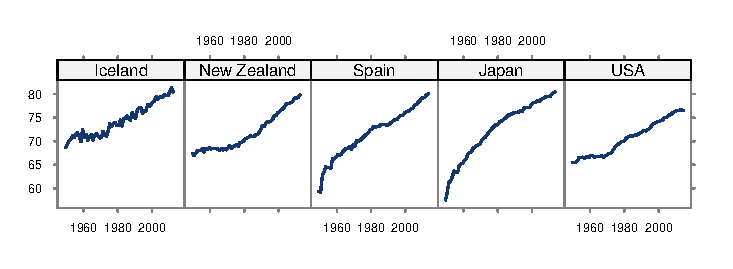
\includegraphics{out/fig_life_exp_sample}
  \caption{Life expectancy at birth.}
\end{subfigure}
\begin{subfigure}{\textwidth}
  \centering
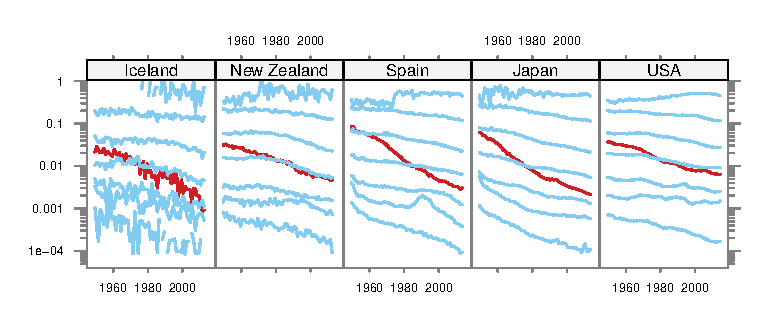
\includegraphics{out/fig_mort_age_sample}
  \caption{Mortality rates.  The rates shown in red are for age 0.  The rates shown in blue are, from bottom to top, for ages 15--19, 30--34, 45--49, 60--64, 75--79, and 100+.}
\end{subfigure}
\caption{Life expectancies and age-specific mortality rates, for males, for 5 selected countries.  The life expectancies come from the Human Mortality Database (HMD) \citep{hmd}. The mortality rates were calculated by us from deaths and exposure data from the HMD.  Life expectancies and mortality rates for females and males for our full sample of 22 countries are shown in Figure XXX of the Extended Data.}
  \label{fig:sample_life_mort}
\end{figure}

\begin{figure}
  \centering
  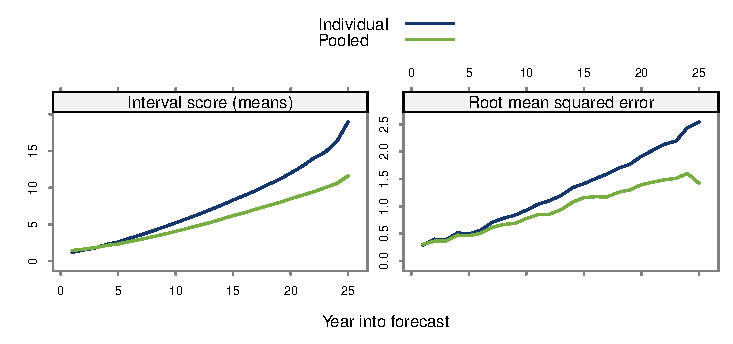
\includegraphics{out/fig_performance_combined}
  \caption{Bla bla}
  \label{fig:performance_combined}
\end{figure}


 


\section*{Methods}
  \label{sec:methods}

% Put methods in here.  If you are going to subsection it, use
% \verb|\subsection| commands.  Methods section should be less than
% 800 words and if it is less than 200 words, it can be incorporated
% into the main text.
  
 

\section{Old notes}
  
        
Importance of understanding mortality change
\begin{itemize}
  \item Basic indicator of social wellbeing; success of health sector etc
  \item Forecasting - pensions, life insurance, population forecasts, aged care, health care
\end{itemize}

Expectations about mortality decline
\begin{itemize}
    \item Lee and Carter, Oeppen and Vaupel etc, pointing out that tapering off in mortality decline not appearing. Governments, demographers systematically understating future declines. 
    \item Has become the new orthodoxy.
    \item Actuaries pointing out that decline slowing - or reversed
    \item Case and Deaton in US
 \end{itemize}


Mortality varies:
\begin{itemize}
  \item Best practice life expectancy follows straight line
  \item Individual country life expectancy not straight lines - slow and fast periods
  \item individual mortality rates even more erratic
 \end{itemize}
 
 Hierarchical models
 \begin{itemize}
   \item despite very large dataset (0.43 billion deaths and  47 billion person-years of observation) have `small sample' problem (paradox of big data)
   \item variability at different levels
   \item for any given country, limited number of years
   \item pool across countries
   \item similar but not identical--hierarchical models
   \item hierarchical models allow us to separate out and model different sources of variability
   \item sample of countries chosen to be approximately exchangeable - makes sense to pool across them
   \item Treat each country as an experiment
 \end{itemize}
 
 We don't focus on sex differences.
 
 
 Age-specific life expectancies deterministic function of age-specific mortality rates
 
  
  
\bibliographystyle{unsrt}
\bibliography{bmort}

\end{document}

